\documentclass[a4paper,twoside,12pt]{book}
%% === nezbytné balíčky:
\usepackage[T1]{fontenc}    % kódování písma
%\usepackage[IL2]{fontenc}  % kódování písma

\usepackage[utf8]{inputenc}     % vstupní znaková sada tohoto dokumentu: UTF-8
%\usepackage[cp1250]{inputenc}  % vstupní znaková sada tohoto dokumentu: Windows 1250
%\usepackage[latin2]{inputenc}  % vstupní znaková sada tohoto dokumentu: ISO Latin 2

\usepackage[english]{babel} % česky psaná práce, typografická pravidla. Překládejte pomocí "latex.exe" nebo "pdflatex.exe"
%\usepackage{czech} % česky psaná práce. Překládejte pomocí "pdfCSlatex.exe" ("cslatex.exe" asi bude mít problém s balíkem geometry)

\usepackage[a4paper, hmarginratio=3:2]{geometry} % využití A4 stránky a nastavení okrajů (u vazby bude širší)

\usepackage{pdfpages} % pokud nemáte formulář "Zadání bak./dipl. práce" naskenovaný jako PDF, tak ZAKOMENTUJTE
\usepackage[hidelinks]{hyperref} % v PDF budou klikací odkazy ("hidelinks" je nebude rámovat)

 \hypersetup{
     colorlinks=true,
     linkcolor=blue,
     filecolor=blue,
     citecolor = black,      
     urlcolor=cyan,
     }

%% === balíčky, které se mohou hodit:
%\usepackage{encxvlna} % postará se o spojky a předložky, které dle českých pravidel nesmí být na konci řádku. Dokumentace: http://texdoc.net/texmf-dist/doc/generic/encxvlna/encxvlna.pdf (chová se správně k "vnitřku" listings?)

\usepackage{graphicx} % balíček pro vkládání rastrových grafických souborů (PNG apod.)
%\usepackage{epsfig} % balíčky pro vkládání grafických souborů typu EPS
%\usepackage{float} % rozšířené možnosti umístění obrázků

%\usepackage{caption} % pro popisky obrázků, tabulek atd.

\usepackage{tabularx} % rozšířené možnosti tabulek
%\usepackage{tabu} % jiný balík pro rozšířené možnosti tabulek

\usepackage{listings}  % balíček vhodný pro ukázky zdrojového kódu v~textu práce/příloh. Nutno nastavit! http://ftp.cvut.cz/tex-archive/macros/latex/contrib/listings/listings.pdf
\usepackage{amsmath} % balíček pro pokročilou matematickou sazbu
%\usepackage{color} % pro možnost barevného textu
%\usepackage{fancybox} % umožňuje pokročilé rámečkování

%\usepackage{index} % nutno použít v případě tvorby rejstříku balíčkem makeindex
%\newindex{default}{idx}{ind}{Rejstřík} % zavádí rejstřík v případě použití balíku index

\usepackage{biblatex}
\addbibresource{sample.bib}

\usepackage{fancyhdr}

\pagestyle{fancy}
\fancyhf{}
\rhead{Overleaf}
\lhead{Guides and tutorials}
\rfoot{Page \thepage}

\graphicspath{{img/}}




\frenchspacing % za větou bude mezislovní mezera (v anglických textech je mezera za větou delší)
\widowpenalty=1000 % "síla" zákazu vdov (= jeden řádek ze začátku odstavce na konci stránky)
\clubpenalty=1000 % "síla" zákazu sirotků (= jeden řádek/slovo z konce odstavce samostatně na začátku stránky)
\brokenpenalty=1000 % "síla" zákazu zlomu stránky za řádkem, který má na konci rozdělené slovo


\topmargin=-15mm      % horní okraj trochu menší
\textwidth=150mm      % šířka textu na stránce
\textheight=240mm     % "výška" textu na stránce


\pagenumbering{arabic} % číslování stránek arabskými číslicemi


\parindent=0pt % odsazení 1. řádku odstavce
\parskip=7pt   % mezera mezi odstavci

\newcommand{\ti}{\textit} % zkrácený příkaz pro kurzívu
\newcommand{\tb}{\textbf} % zkrácený příkaz pro tučné písmo


%% --- zde jsou zavedeny některé "konstanty" - některé musíte změnit! --- %%
\newcommand{\cvut}{Tertiary Professional School, Secondary School}
\newcommand{\fjfi}{The Centre of professional training Sezimovo Ústí}
\newcommand{\program}{Electrotechnics}

\newcommand{\obor}{Mechatronic systems} % změňte, pokud máte jiný obor

\newcommand{\druh}{Thesis} % nebo "Diplomová práce"
\newcommand{\woman}{} % pokud jste ŽENA, ZMĚŇTE na: ...{\woman}{a} (je to do Prohlášení)

\newcommand{\logoCVUT}{
\includegraphics{copsu_logo.jpg}} % logo ČVUT -- podle grafického manuálu ČVUT platného od prosince 2016. Pokud nevyhovuje PDF-verze, tak použijte jinou variantu loga: https://www.cvut.cz/logo-a-graficky-manual -> "Symbol a logo ČVUT v Praze"). Pokud chcete logo úplně vynechat, zadejte místo "\includegraphics{...}" text "\vspace{35mm}"

% přesně podle formuláře "Zadání bak./dipl. práce" VYPLŇTE:
\newcommand{\nazevcz}{Postprocesor robota pro metodu Laser Shock Peening}    % český název práce (přesně podle zadání!)
\newcommand{\nazeven}{Robot post processor for Laser Shock Peening technique}          % anglický název práce (přesně podle zadání!)
\newcommand{\autor}{Marek Böhm}   % vyplňte své jméno a příjmení (s akademickým titulem, máte-li jej)
\newcommand{\vedouci}{Mgr. Bc. Miroslav V. Hospodářský} % vyplňte jméno a příjmení vedoucího práce, včetně titulů, např.: Doc. Ing. Ivo Malý, Ph.D.
\newcommand{\pracovisteVed}{VOŠ, SŠ, COP Sezimovo Ústí} % ZMĚŇTE, pokud vedoucí Vaší práce není z KSI
\newcommand{\konzultant}{Ing. Jakub Horáček} % POKUD MÁTE určeného konzultanta, NAPIŠTE jeho jméno a příjmení
\newcommand{\pracovisteKonz}{HiLASE centrum, Fyzikální ústav AV ČR, v. v. i.} % POKUD MÁTE konzultanta, NAPIŠTE jeho pracoviště

% podle skutečnosti VYPLŇTE:
\newcommand{\rok}{2021}  % rok odevzdání práce (jen rok odevzdání, nikoli celý akademický rok!)
\newcommand{\kde}{Sezimovo Ústí} % studenti z Děčína ZMĚNÍ na: "Děčíně" (doplní se k "prohlášení")

\newcommand{\klicova}{RoboDk, Industrial Robots, Robotic Arms, Collision Avoidance, Simulation, Post processor}   % zde NAPIŠTE česky max. 5 klíčových slov
\newcommand{\keyword}{RoboDk, Industrial Robots, Robotic Arms, Collision Avoidance, Simulation, Post processor}       % zde NAPIŠTE anglicky max. 5 klíčových slov (přeložte z češtiny)
\newcommand{\abstrCZ}{Popis práce česky}    % zde NAPIŠTE abstrakt v češtině (cca 7 vět, min. 80 slov)
\newcommand{\abstrEN}{
The focus of this thesis is to develop a post-processor for the Laser Shock Peening Technique. 

This thesis seeks to answer the following thing: How can a post-processor be altered to use it for the Laser Shock Peening Technique. 

The RoboDK CAM program is a powerful tool that enables users to create their post-processors. In this thesis, the process of modifying a post-processor is described. The post-processor is then tested on a real industrial robotic arm.

} % zde NAPIŠTE abstrakt v angličtině

\newcommand{\prohlaseni}{I declare that I have prepared my thesis independently, and I have used only the materials (literature, projects, software, etc.) listed in the attached list.} % text prohlášení můžete mírně upravit :-)

\newcommand{\podekovani}{I want to thank my supervisor Mgr. Bc. Miroslav V. Hospodářský for the invaluable advice and help in creating this thesis.} % NAPIŠTE poděkování, např. svému vedoucímu:
% Děkuji Ing. Eleonoře Krtečkové, Ph.D. za vedení mé bakalářské práce a za podnětné návrhy, které ji obohatily.
% NEBO:
% Děkuji vedoucímu práce doc. Pafnutijovi Snědldítětikaši, Ph.D. za neocenitelné rady a pomoc při tvorbě bakalářské práce.

\begin{document}
%%%%%%%%%%%% TITULNÍ STRANA -- na následujících cca 30 řádků NESAHEJTE!!!  Generuje se AUTOMATICKY %%%%%%%%%%%%
\thispagestyle{empty}

\begin{center}
	{\LARGE
		\cvut\par
		\fjfi
	}
    \vspace{10mm}

    \begin{tabular}{c}
		\tb{Program: \program}  \\[3pt]   
		\tb{Specialization: \obor}\\
    \end{tabular}

   \vspace{10mm} \logoCVUT \vspace{15mm} 

   {\huge \tb{\nazevcz}\par}
   \vspace{5mm}   
   {\huge \tb{\nazeven}\par}
   
   \vspace{15mm}
   {\Large \MakeUppercase{\druh}}

   \vfill
   {\large
    \begin{tabular}{ll}
    Author : & \autor\\
    Supervisor: & \vedouci\\
    Year: & \rok
    \end{tabular}
   }
\end{center}

\clearpage{\pagestyle{empty}\cleardoublepage} % prázdná stránka za tou "titulní", bez čísla

%%%%%%%%%%%% ZADÁNÍ PRÁCE %%%%%%%%%%%%
% Zadání (podepsané děkanem!) musíte NASKENOVAT. Ideálně jako 2stránkové PDF (soubor "zadani_cele.pdf"). 
% Před svázáním to v jednom výtisku VYMĚNÍTE ZA ORIGINÁLNÍ ZADÁNÍ (podepsané děkanem fakulty)!
\newpage  % SEM NESAHEJTE!
\thispagestyle{empty} % SEM NESAHEJTE!

%% zde podle toho, jak jste zadání naskenovali, VYBERTE variantu A, B nebo C:
%
% --- varianta A: zadání naskenované jako 2stránkové PDF:
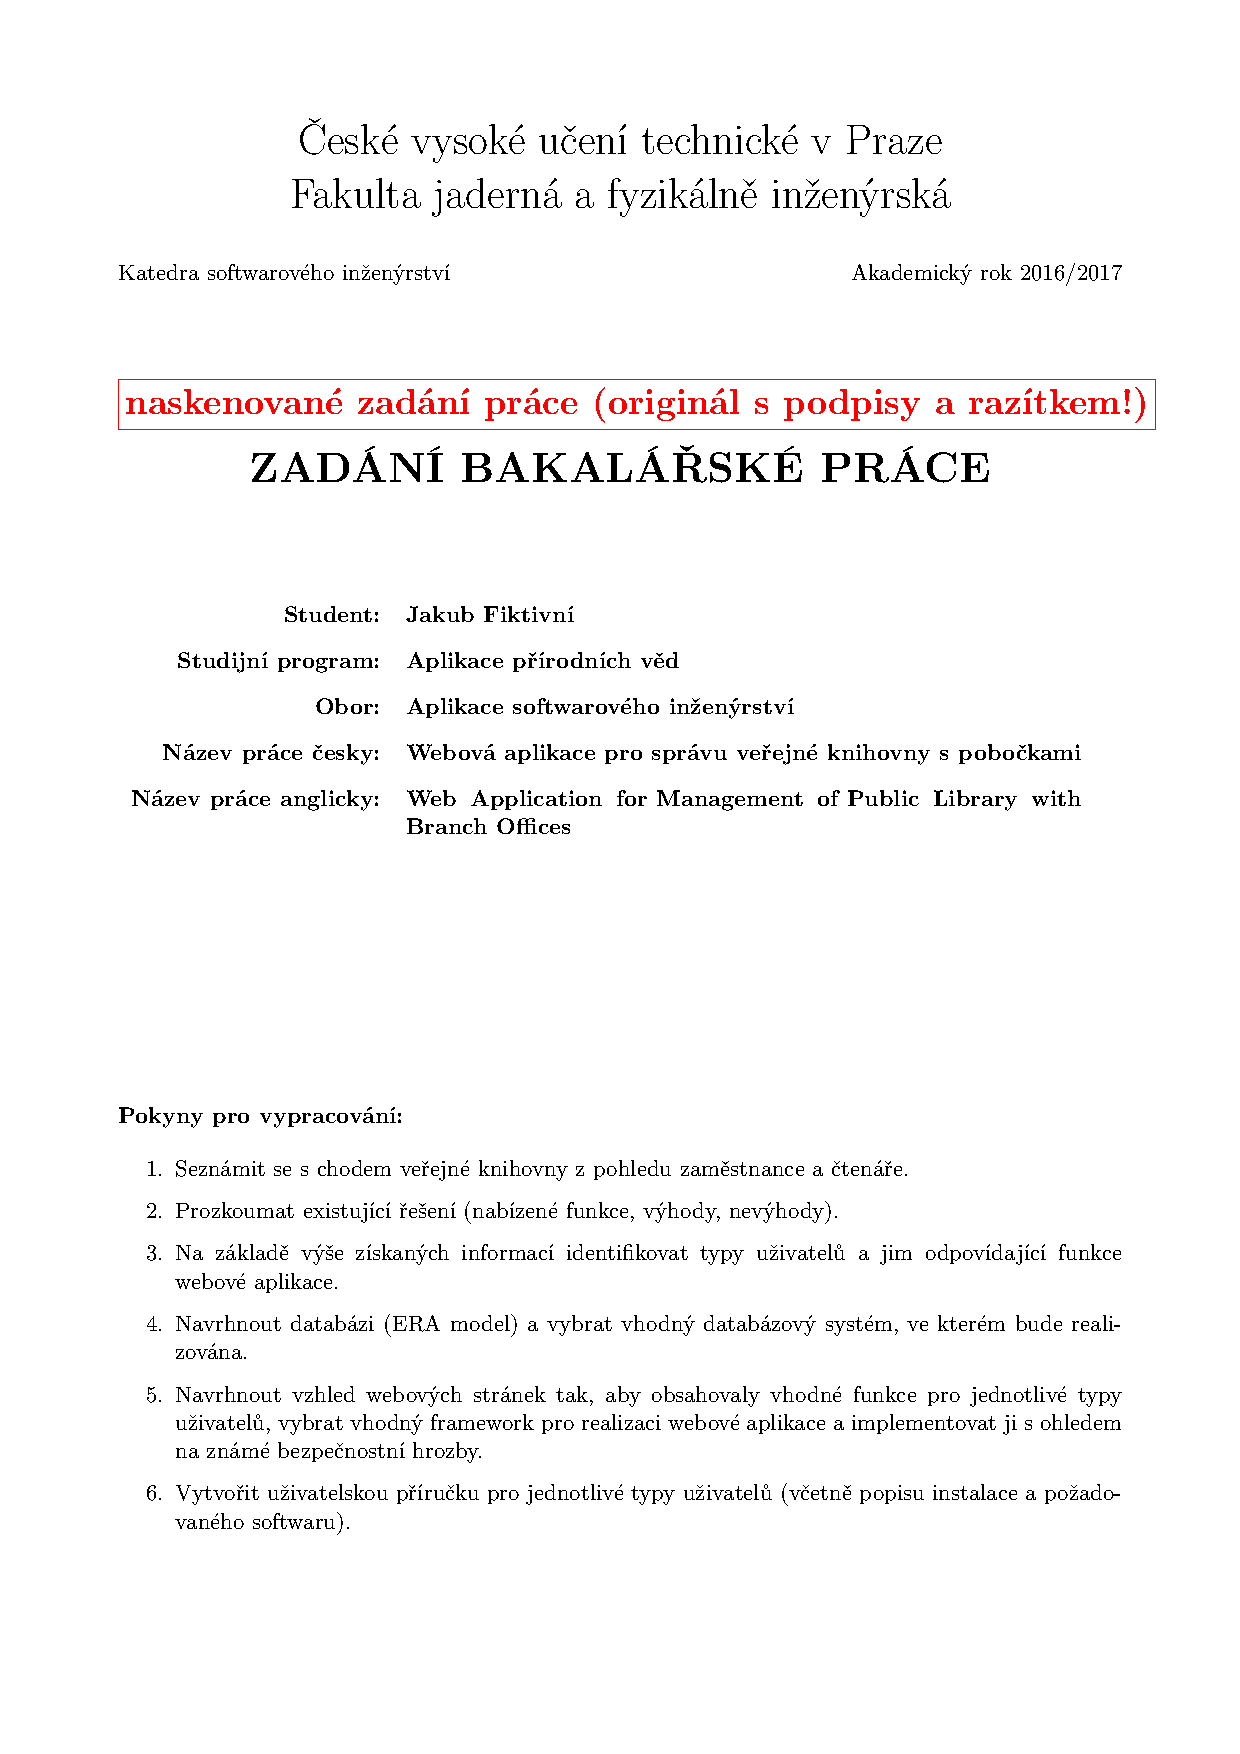
\includepdf[pages={1,2}]{zadani_cele.pdf} % NAHRAĎTE správným souborem!
%
%% --- varianta B: zadání naskenované jako jednotlivé stránky:
%\includepdf[pages={1}]{zadani1.pdf} % 1. strana zadání v PDF
%\includepdf[pages={1}]{zadani2.pdf} % 2. strana zadání v PDF
%
%% --- varianta C: zadání naskenované jako 2 samostatné obrázky:
%% 1. strana zadání
%\begin{center}
%     \includegraphics[width=1\textwidth]{zadani1.jpg}
%\end{center}
%% 2. strana zadání
%\newpage  % SEM NESAHEJTE!
%\thispagestyle{empty} % SEM NESAHEJTE!
%\begin{center}
%     \includegraphics[width=1\textwidth]{zadani2.jpg}
%\end{center}


%%%%%%%%%%%% Prohlášení -- SEM NESAHEJTE! Generuje se automaticky z výše nastavených maker \kde{} a \prohlaseni{}. %%%%%%%%%%%%
\newpage % SEM NESAHEJTE!
\thispagestyle{empty}  % SEM NESAHEJTE!

~ % SEM NESAHEJTE!
\vfill % prázdné místo. SEM NESAHEJTE!

\tb{Declaration} % SEM NESAHEJTE!

\vspace{1em} % vertikální mezera. SEM NESAHEJTE!
\prohlaseni

\vspace{2em}  % SEM NESAHEJTE!
\hspace{-0.5em}\begin{tabularx}{\textwidth}{X c}  % SEM NESAHEJTE!
In \kde\ on .................... &........................................ \\	% SEM NESAHEJTE!
	& \autor
\end{tabularx}	% SEM NESAHEJTE!


%%%%%%%%%%%% Poděkování  %%%%%%%%%%%%
\newpage
\thispagestyle{empty}

~
\vfill % prázdné místo


% -- následující kus kódu (do "%%%%%%%%%%%% ABSTRAKT") můžete odstranit, pokud nechcete psát poděkování:
\tb{Acknowledgments}

\vspace{1em} % vertikální mezera
\podekovani
\begin{flushright}
\autor
\end{flushright}  % <------- tady končí stránka s poděkováním


%%%%%%%%%%%% ABSTRAKT atp. Je generován AUTOMATICKY podle maker nastavených na začátku souboru) %%%%%%%%%%%% 
\newpage   % SEM NESAHEJTE!
\thispagestyle{empty}   % SEM NESAHEJTE!

% příprava:    (na následujících 8 řádků NESAHEJTE!)
\newbox\odstavecbox
\newlength\vyskaodstavce
\newcommand\odstavec[2]{%
    \setbox\odstavecbox=\hbox{%
         \parbox[t]{#1}{#2\vrule width 0pt depth 4pt}}%
    \global\vyskaodstavce=\dp\odstavecbox
    \box\odstavecbox}
\newcommand{\delka}{120mm} % šířka textů ve 2. sloupci tabulky

% použití přípravy:    % dovnitř "tabular" vůbec NESAHEJTE!
\begin{tabular}{ll}
  {\em Název práce:} & ~ \\
  \multicolumn{2}{l}{\odstavec{\textwidth}{\bf \nazevcz}} \\[1em]
  {\em Autor:} & \autor \\[1em]
  {\em Studijní program:} & \program \\
  {\em Obor:} & \obor \\
  {\em Druh práce:} & \druh \\[1em]
  {\em Vedoucí práce:} & \odstavec{\delka}{\vedouci\\ \pracovisteVed} \\
  {\em Konzultant:} & -- %\odstavec{\delka}{\konzultant \\ \pracovisteKonz}  % VYMAŽTE text "-- %" v případě, že jste neměli konzultanta
 \\[1em]  
  \multicolumn{2}{l}{\odstavec{\textwidth}{{\em Abstrakt:} ~ \abstrCZ  }} \\[1em]
  {\em Klíčová slova:} & \odstavec{\delka}{\klicova} \\[2em]

  {\em Title:} & ~\\
  \multicolumn{2}{l}{\odstavec{\textwidth}{\bf \nazeven}}\\[1em]
  {\em Author:} & \autor \\[1em]
  \multicolumn{2}{l}{\odstavec{\textwidth}{{\em Abstract:} ~ \abstrEN  }} \\[1em]
  {\em Key words:} & \odstavec{\delka}{\keyword}
\end{tabular}



%%%%%%%%%%%% Obsah práce ... je generován AUTOMATICKY %%%%%%%%%%%%
\newpage  % SEM NESAHEJTE!
\parskip=0pt
\tableofcontents % SEM NESAHEJTE!
\parskip=7pt
\newpage % SEM NESAHEJTE!


%--------------------------------------------------------
%|         Zde začíná SAMOTNÁ PRÁCE (text)              |
%--------------------------------------------------------

\chapter*{Introduction} % SEM NESAHEJTE!
\addcontentsline{toc}{chapter}{Introduction} % SEM NESAHEJTE!
%
Zde napište text úvodu (1-3 strany, nerozdělujte na podkapitoly) nebo jej vložte ze samostatného souboru: např. příkazem \texttt{\textbackslash input\{vnitrek\_uvod.tex\}}. \cite{einstein}
%
%\input{vnitrek_uvod.tex}



\chapter{Basics of Robotics}
%

%
%\input{vnitrek_kapitola1.tex} % text vkládán ze souboru. Pokud je v souboru uveden i příkaz \chapter{...}, tak ho o 4 řádky výše vymažte.

\section{Industrial robots}


\chapter{Chapter 3 - Design}

\section{RoboDK}

RoboDK is a development platform for industrial robot offline programming and simulation.

\subsection{RoboDK history}

RoboDK (the company) was founded by Albert Nubiola and Lauren Ierullo in January 2015 as a spin-off company from the \href{https://en.etsmtl.ca/unites-de-recherche/coro/accueil?lang=en-CA}{CoRo laboratory}   at ETS University in Montreal, Canada. RoboDK is a commercial version of RoKiSim, a multi-platform educational software tool for 3D simulation of serial six-axis robots.

\subsection{RoboDK features}

RoboDK is a CAM (Computer-aided manufacturing) simulator for industrial robots and robot programming. Mobile robots are not supported. 

RoboDK supports offline programming and has an extensive robot library supporting many robot controllers, including:

\begin{itemize}
    \item ABB RAPID (mod/prg)
    \item Fanuc LS (LS/TP)
    \item KUKA KRC/IIWA (SRC/java)
    \item Motoman Inform (JBI)
    \item Universal Robots (URP/script)
\end{itemize}

RoboDK offers a free (limited), educational or professional version. 
The software is available for Windows, Mac OS, Ubuntu Linux or Android. It supports either 32 or 64-bit versions of the abovementioned operating systems. At the time of writing this document, the latest version of RoboDK is 5.2.The logo of RoboDK is shown in Figure \ref{fig:robodklogo}.

\begin{figure}[h]
    \centering
    
\includegraphics[width=0.6\linewidth]{img/robodk_logo.png}
    \caption{RoboDK logo.}
    \label{fig:robodklogo}
\end{figure}

\subsection{RoboDK interface}

The interface of RoboDK consists of the main menu, the toolbar, the station tree, the status bar and the 3D view. A picture of the RoboDK interface is shown in Figure \ref{fig:robodkinterface}. An extensive documentation for RoboDK is available \href{https://robodk.com/doc/en/Basic-Guide.html#Start}{online}.


\begin{figure}[h]
    \centering
    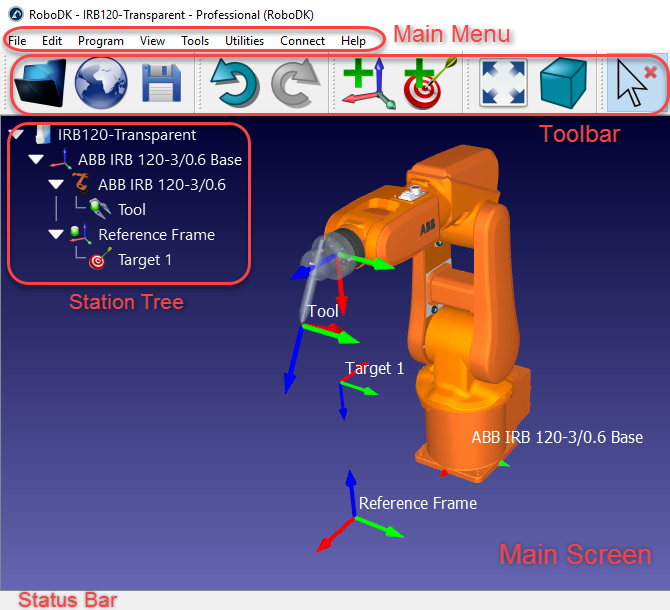
\includegraphics[width=0.6\linewidth]{img/robodk_interface.png}
    \caption{RoboDK interface.}
    \label{fig:robodkinterface}
\end{figure}

\subsection{RoboDK API}



\chapter*{Závěr} % SEM NESAHEJTE!
\addcontentsline{toc}{chapter}{Závěr} % SEM NESAHEJTE!
%
Zde napište text úvodu (1-3 strany, nerozdělujte na podkapitoly) nebo jej vložte ze samostatného souboru: např. příkazem \texttt{\textbackslash input\{vnitrek\_zaver.tex\}}.
%
%\input{vnitrek_zaver.tex}


%%%%%%%%%%%% SEZNAM POUŽITÝCH ZDROJŮ (LITERATURA) %%%%%%%%%%%%
\clearpage  % SEM NESAHEJTE!
\addcontentsline{toc}{chapter}{Literatura} % SEM NESAHEJTE!

\begin{thebibliography}{99}   
	% formát: ČSN ISO 690. Můžete si to vygenerovat na http://www.citacepro.com (přihlaste se přes odkaz "ČVUT"), umí to vygenerovat TeX
	% řazení: abecedně podle autora (resp. prvního slova, není-li znám autor)
	\bibitem{odkaz} Autor. \ti{Název knihy}. Město. Nakladatelství. Rok.  
\end{thebibliography}


%%%%%%%%%%%% PŘÍLOHY PRÁCE %%%%%%%%%%%%
\newpage % SEM NESAHEJTE!
\addcontentsline{toc}{chapter}{Přílohy} % SEM NESAHEJTE!
\appendix % SEM NESAHEJTE!


%%%%%%%%%%%% Příloha A (tj. 1. kapitola v rámci příloh) %%%%%%%%%%%%




\printbibliography


\end{document} % SEM NESAHEJTE! Konec.
